\documentclass[a4paper,12pt]{article} %indique la classe du document, et les options

\pagenumbering{arabic}
%le pr\'eambule
\usepackage[french]{babel}
\usepackage{graphicx}
\usepackage{array}


%Titre
\makeatletter
\def\clap#1{\hbox to 0pt{\hss #1\hss}}%
\def\ligne#1{%
\hbox to \hsize{%
\vbox{\centering #1}}}%
\def\haut#1#2#3{%
\hbox to \hsize{%
\rlap{\vtop{\raggedright #1}}%
\hss
\clap{\vtop{\centering #2}}%
\hss
\llap{\vtop{\raggedleft #3}}}}%
\def\bas#1#2#3{%
\hbox to \hsize{%
\rlap{\vbox{\raggedright #1}}%
\hss
\clap{\vbox{\centering #2}}%
\hss
\llap{\vbox{\raggedleft #3}}}}%
\def\maketitle{%
\thispagestyle{empty}\vbox to \vsize{%
\haut{\includegraphics[width=0.35\linewidth]{../../Newcastle-University.jpg}}{\vspace{1cm}\@blurb}{}
\vfill
\vspace{1cm}
\begin{flushleft}
\usefont{OT1}{ptm}{m}{n}
\huge \@title
\end{flushleft}
\par
\hrule height 4pt
\par
\begin{flushright}
\usefont{OT1}{phv}{m}{n}
\Large \@author 
\normalsize \@student
\par
\end{flushright}
\vspace{1cm}
\center
\includegraphics{Metro-Wiki-logo.png}
\vfill
\vfill
\bas{}{\@location, le \@date}{}
}%
\cleardoublepage
}
\def\date#1{\def\@date{#1}}
\def\author#1{\def\@author{#1}}
\def\title#1{\def\@title{#1}}
\def\location#1{\def\@location{#1}}
\def\student#1{\def\@student{#1}}
\def\blurb#1{\def\@blurb{#1}}
\date{\today}

\makeatother
\title{
Usability Analysis : \\ Tyne and Wear Metro Ticket machines
}
\author{Nicolas Desfeux}
\student{(Erasmus Student n\degre110477367)}
\location{Rennes}

\blurb{
Newcastle University\\
\textbf{School of Computing Science}\\[1em]
CSC3003 : Interaction Design
}
%document principal 

\begin{document}
\maketitle
\newpage
\tableofcontents
\newpage
\section*{Introduction}
\addcontentsline{toc}{section}{Introduction}
\paragraph{}The Tyne and Wear is a rail system standing in the North East of England since 1980. Nowadays, this Metro is use for more than 100,000 daily ridership, over sixty stations. To use this Metro, people have to use tickets. In every station, you can find machines that allow you to buy tickets. There is not only one ticket, and several purchase options are available. In this documents, we'll first discuss the accessibility and the usability of those machines. Then we'll try to provide a new design, according to the notions we studied in this module.
\section{Usability and accessibility of the Tyne and Wear Metro Tickets machine}
\paragraph{}This section will describe and study the actual tickets machine available in Tyne and Wear Metro stations in Newcastle. The figure \ref{machine} shows you a picture of the actual tickets machine.
\begin{figure}[h!]
\center 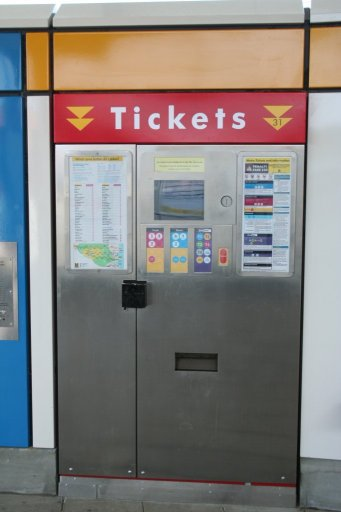
\includegraphics[width=0.35\linewidth]{metro.jpg}
\caption{\label{machine} Tyne and Wear Metro Tickets machine}
\end{figure}
\paragraph{}The machines is kind of a big box, with a screen, some buttons under it, some reading on the sides and a compartment for collecting ticket.
\subsection{Goals}
The purpose of the machine is to provided tickets for the Metro train station. Several kind of tickets are available. There are two options for a ticket : the destination you want to go, and the validity time of your ticket. The machine might be able to set those options, and provided the good tickets.
\subsection{Usability}
\subsubsection{Niel's principles}
\subsubsection{Dix et al's usability principles}
\subsection{Accessibility analysis}
\subsubsection{Perceptibly}
\paragraph{Information presentation : }All the informations are displayed with text, and colored buttons. There are 3 display zones : 
\begin{itemize}
\item The screen  : The actual screen display informations in two colors : black background, and orange-yellow writing.
\item Metro lines on the left : This shows where the stations are and explains the zones system.
\item General informations on the right : It explains the rules of the rail system, what is allowed and not, ...
\end{itemize}
Under the screen, you can find the buttons for tickets selection.  Buttons are organized to help people easily find the ticket they want.
\paragraph{Assistive technologies} It doesn't seems to have help for people. There is no way to zoom on the screen, and buttons look quiet the same. There is no depth system, for example headphones support, that could help people.
\subsubsection{Operability}
\paragraph{Action needed : } To get a ticket, three actions are needed : 
\begin{enumerate}
\item Click on the button corresponding to the ticket you want to purchase (one of the button below the screen).
\item Insert the coins (and only coins !) corresponding to the price of the ticket.
\item Get your ticket and your change from the collecting box, below the buttons.
\end{enumerate}
That's only three actions. The ticket selection might be quiet confusing. To pay for your ticket, you can only uses coins. No notes and cards payments are allowed, which can be quiet annoying for the user. The price is displayed on the screen. Theres is no way to get several tickets on the same set of commands. You have to start again to have an other ticket, even if it's the same at the first.

We also study users input and output : 
\paragraph{Money}
\paragraph{Collecting box}
We also study users input and output : 
To collect your ticket, you have to a "door" on the machine, where the ticket is released. Most people need to do an extra movement to collect the tickets, and going close to the ground. It's not that easy to see what's in the box when you're standing up.

\subsubsection{Simplicity}
The simplicity of this machine is quiet obvious.

\subsubsection{Forgiveness}
During the execution of the three action, only the two first need to allow forgiveness. There is, below the screen, a cancel button. If you are executing one of the first two actions, pushing this button cancel everything was begin (remove ticket selection, giving money back if coins was inserted).

\subsubsection{Output}


\subsection{Issues summarize}
Even if those machine achieve the goal they are asking for, and some of the design used are quiet efficient, there are some issues that we can point out.
Here are some issues that we found about this new machine : 
\begin{itemize}
\item Collecting box position
\item Payment only by cash
\item Screen position and display
\end{itemize}

\section{Redesigning  of the Tyne and Wear Metro Tickets machine}
\subsection{Requirement specifications}
\subsection{Physical description}
\begin{figure}[h!]
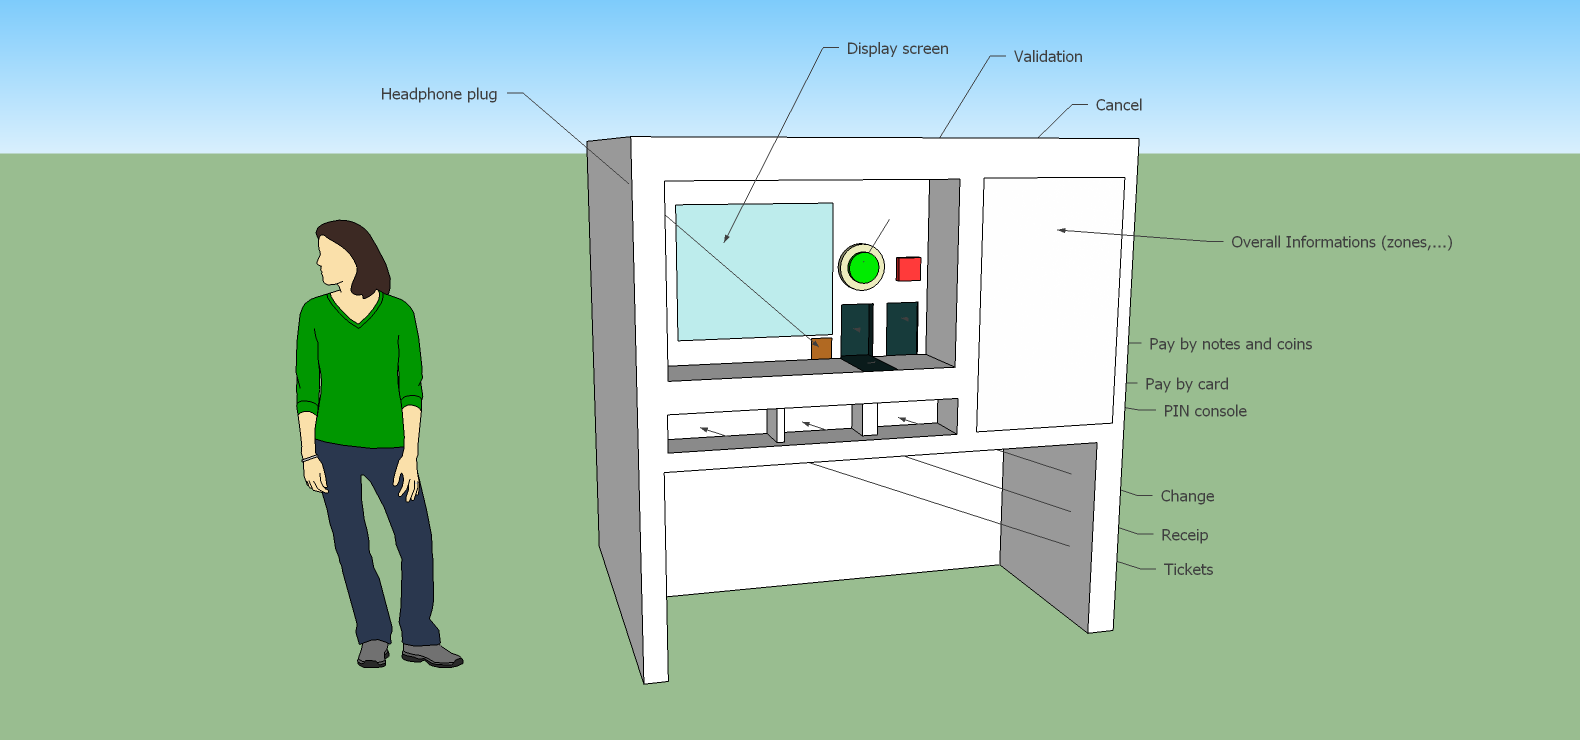
\includegraphics[width=1.3\linewidth]{ID.png}
\caption{\label{new} Tyne and Wear Metro Tickets machine, new design}
\end{figure}
\begin{figure}[h!]
%\includegraphics[width=1.3\linewidth]{screen.png}
\caption{\label{new} Tyne and Wear Metro Tickets machine, user interface}
\end{figure}
\subsubsection{input}
Buttons  rotative button, cancel button, validation.
Card : cards insertion, pin code.
Change : coins and notes
headphones : Nothing around it.
\subsubsection{output}
Screen
Tickets
Receip
Change
Sounds
\subsection{Software design}
options seprations.


\newpage
\section*{Conclusion}
\addcontentsline{toc}{section}{Conclusion}
\paragraph{}The actual metro tickets station that you find in Newcastle clearly have some issues, for classic users (no notes, no cards, ...), and for people with disability (position and size of the machine, no handle of headphones,...). For most of people, those issues are transparent, but they still exist, and some people can have real trouble getting a ticket.
\paragraph{}Designing a new Metro tickets machine is not that easy when you try to fix all of that issue. However, lying on the principle we saw in lectures, we manage to create a machine more usable and accessible for passengers. To be sure of that, the next step would doing an evaluation of this design. The evaluation would help validate (and correct if needed) the design we made. 

\newpage
\nocite{Org}
\nocite{Wikipedia}
\bibliographystyle{abbrv}
\bibliography{main}
\end{document}
This is never printed